
\chapter{Introducci\'on}\label{capit:cap1}
\vspace{-2.0325ex}%
\noindent
\rule{\textwidth}{0.5pt}
\vspace{-5.5ex}% 
\newcommand{\pushline}{\Indp}


Actualmente la poblaci\'on de adutos mayores va en aumento. Cuando sufren de enfermedades o padecimiento es que com\'un que necesiten de servicios de cuidadores. Los cuidadores por su parte, sufren de problemas derivados de su labor. En un estudio, 60\% de los cuidadores desarrollaron un desorden depresivo y/o de ansiedad en los primeros 24 meses: 37\% de depresi\'on, 55\% desorden de ansiedad y 32\% ambos. \citep{Joling2014}.Este mismo problema se ve tambi\'en en los cuidadores de personas con demencia.  Casi un cuarto de ellos tienen un nivel de ansiedad cl\'inico significante \citep{Cooper200615}.

	En este trabajo, se explora la utilidad del c\'omputo vestible (computadoras lo suficientemente peque\~nas para ser usadas como ropa) como herramienta para la detecci\'on de ansiedad en cuidadores de personas con demencia. Se muestra el dise\~no de un experimento para recabar datos que ayuden a la detecci\'on de ansiedad y los resultados de la detecci\'on utilizando aprendizaje de m\'aquina.
	
	
	
	%	Casi un cuarto de ellos tienen un nivel de ansiedad cl\'inico significante \citep{Cooper200615}. Mientras que la carga de los cuidadores informales aumenta, se vuelve mas probable que sufran de ansiedad y depresi\'on \citep{Denno20131731}. La carga en los cuidadores (f\'isica o psicol\'ogica) podr\'ia aumentar los niveles de ansiedad. Entre mas demandante es un servicio, mayor podr\'ia ser la ansiedad percibida. 
	
	

	
	%Los comportamientos bizarros o impredecibles de la persona afectada por demencia aumentan la carga emocional \citep{Rosa201054}. En este estudio, se har\'a uso del c\'omputo vestible para capturar informaci\'on de ansiedad y se utilizar\'a aprendizaje de m\'aquina para detectar periodos de ansiedad en cuidadores de personas con demencia.

	%La demencia es un s\'indrome del declive de las habilidades cognitivas. Los s\'intomas comunes son: problemas de memoria, dificultades para realizar tareas, mal juicio, deterioro del lenguaje hablado y cambios de humor\citep{Aziz}. Afecta alrededor del 4\% de las personas mayores de 65 a\~nos y al 40\% de las personas mayores de 90. 
\section{Plantamiento del problema}
	Se encuentra documentado que los cuidadores sufren de problemas de ansiedad, estr\'es y depresi\'on. A pesar de que se ha demostrado en otros estudios la capacidad de utilizar sensores de datos fisiol\'ogicos para detectar ansiedad, no se ha abordado el problema de los cuidadores de personas con demencia. Los retos para recabar datos de estas situaciones son variados. Tener certeza que la persona se encuentra en un estado ansioso y la captura de datos fisiol\'ogicos en situaciones naturales son los retos mas significativos. En este trabajo, se propone un experimento para solventar estos problemas.
\section{Objectivos}
	A continuaci\'on se listan los objetivos de este trabajo.
\subsection{Objetivo general}
	Detectar periodos de ansiedad en cuidadores de personas con demencia por medio de c\'omputo vestible
\subsection{Objetivos espec\'ificos}
	Dise\~nar un experimento para la detecci\'on de ansiedad en cuidadores de personas con demencia
\subsection{Hip\'otesis de investigaci\'on}
	?`Como pueden los dispositivos vestibles ayudar a la detecci\'on de ansiedad en cuidadores de personas con demencia?
\subsection{Propuesta de la soluci\'on}
	Se propone dise\~nar un experimento para recabar datos de ansiedad en cuidadores de persona con demencia en situaciones naturalistas. Los datos recabados son datos fisiol\'ogicos del participante. Adem\'as se utilizar\'an datos en forma de video, autoreportado y observaci\'on para determinar en que situaciones el participante siente los periodos de ansiedad. Por \'ultimo, se utilizar\'an t\'ecnicas de aprendizaje de m\'aquina para mostrar la posibilidad de utilizar estos datos para la detecci\'on de ansiedad.

\section{Metodolog\'ia}\label{secc:methodology}
La metodolog\'ia seguida se bas\'o en tres pasos: \textit{Captura de datos}, \textit{Detecci\'on de ansiedad}, y un paso hipot\'etico de \textit{Estrategias de afrontamiento} (ver figura ~\ref{fig:metodology}). El primer paso consiste en recabar informaci\'on de cuidadores bajo situaciones de ansiedad con el fin de etiquetar eventos. Esta captura se logr\'o por medio de un experimento que implementa una t\'ecnica de ``Naturalistic Enactment''.  Los eventos ser\'an clasificados como de ansiedad y no ansiedad. Se segmentar\'an las se\~nales en periodos de 30 segundos y se extraer\'an las caracter\'isticas de las porciones de las se\~nales correspondientes. Los datos ser\'an procesados con utiler\'ias ya programadas en python. Una vez capturada y etiquetada la informaci\'on, se desarroll\'o un m\'etodo basado en t\'ecnicas de aprendizaje de m\'aquina que tom\'o los segmentos de ansiedad. El tercer paso, aunque queda fuera del alcance de esta tesis se discute como las posibles aplicaciones por medio de tecnolog\'ia m\'ovil y/o pantallas ambientales.
\begin{figure}[h!]
        \centering
        \subfigure[]{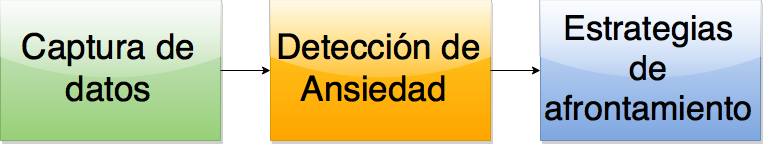
\includegraphics[width=160mm]{./Figures/img_metodologia}}
        \caption{Metodolog\'ia seguida durante la investigaci\'on.} \label{fig:metodology}
\end{figure}
\subsection{Contribuci\'on}
	En la actualidad, no existen intervenciones no tecnol\'ogicas para detectar la ansiedad en cuidadores de personas con demencia. Estas intervenciones tradicionales se basan en el uso de encuestas y cuestionarios y actuan sobre periodos de tiempo muy largos. Este trabajo se basa en la detecci\'on de ansiedad situacional, que permite conocer con mas a detalle la frecuencia de estos eventos.
	Adem\'as, se generar\'a una base de datos de eventos de ansiedad que permitir\'a realizar pruebas de t\'ecnicas de detecci\'on de ansiedad que surgan en el futuro.
\subsection{Conclusi\'on}
	Se encuentra documentada a la ansiedad como un problema que enfrentan los cuidadores de personas con demencia. Con la tendencia en el aumento de la poblaci\'on de adultos mayores, se espera que el n\'umero de cuidadores aumente por lo que es necesario tomar en cuenta las necesidades de este sector. Con la tendencia en el uso de dispositivos vestibles capaces de sensar el ambiente del usuario, la detecci\'on de ansiedad por medio de c\'omputo vestible se vuelve una opci\'on para mejorar la calidad de vida de los cuidadores.

\section{Pregunta de investigac\'ion}
	?`C\'omo pueden los dispositivos vestibles ayudar a detectar ansiedad en cuidadores de personas con demencia?
\section{Hip\'otesis}
	\begin{itemize}
	\item{Los sujetos tendr\'an mayores valores en las caracter\'isticas de GSR y EEG durante un periodo de ansiedad alto que durante uno bajo.}
	\item{Los sujetos tendr\'an mayor valor HR promedio durante un periodo de ansiedad alto que durante uno bajo}
	\item{Los sujetos que reporten mayores valores en la prueba de SUDS tendr\'an mayores valores en las caracter\'isticas de GSR, HR, y EEG durante un periodo de ansiedad.}
	\end{itemize}
\section{Variables independientes}
	\begin{itemize}
		\item{Periodos con ansiedad}
		\item{Periodos sin ansiedad}
	\end{itemize}
\section{Variables dependientes}
	\begin{itemize}
		\item{Caracter\'isticas de GSR: N\'umero de picos por segmento, Amplitud y tiempo de recuperaci\'on medio}
		\item{Valor de HR: Promedio de HR}
	\end{itemize}
\section{Escenario}
	Los participantes ser\'an transportados del departamento de computaci\'on de CICESE hacia una casa donde se encontrar\'a el adulto mayor
	para realizar la prueba.
	Se les pedir\'a reposar durante 15 minutos en el lugar para regularizar su sudoraci\'on y ritmo cardiaco.
	Luego, se les tomar\'a una muestra de 5 minutos de sus se\~nales fisiol\'ogicas como l\'inea base por medio de una banda para HR, una pulsera para GSR y una diadema para EEG. Durante estos 5 minutos
	se les pedir\'a  que reposen sentados en una habitaci\'on sin el adulto mayor y con los ojos cerrados, concetr\'andose en su respiraci\'on como t\'ecnica de relajaci\'on.

	Pasado el tiempo de relajaci\'on se les presentar\'a al adulto mayor en una habitaci\'on diferente.Despu\'es de la introducci\'on llevar\'an a cabo la terapia. Una vez mas, llevar\'an sobre el cuerpo la banda de ritmo cardiaco, la pulsera para GSR y la diadema de EEG. Durante la prueba, se les pedir\'a que reporten su nivel de ansiedad por medio de un formato especial.

\section{Configuraci\'on del escenario}
	
	Los datos ser\'an capturados de la siguiente manera:
	\begin{itemize}
		\item{La se\~nal de suduraci\'on se obtendr\'a por medio de la pulsera \textbf{Empatica E3} que ser\'a conectada a un tel\'efono inteligente Samsung S4 con android 4.0 ejecutando la aplicaci\'on CareMeToo hecha en el laboratorio.}
		\item{La se\~nal de ritmo cardiaco se obtendr\'a por medio de una banda zephyr HxM conectado a una macbook 2008 ejecutando la aplicaci\'on \textbf{anxiLogger} hecha en el laboratorio.}
		\item{La se\~nal de EEG se obtendr\'a por medio de la diadema Muse conecatada a la misma macbook 2008 ejecutando la aplicaci\'on Muse Lab.}
		\item{Todo el procedimiento ser\'a grabado por medio de una c\'amara Sony HD instalada en el lugar.}
	\end{itemize}
\section{Consideraciones}
	\begin{itemize}
		\item{Los participantes no podr\'an tomar bebidas con cafe\'ina (caf\'e, t\'e, refresco, bebidas energ\'eticas etc.) durante al menos 8 horas antes de la prueba.}
		\item{Los participantes no podr\'an interactuar con los investigadores una vez que inicie la prueba.}
		\item{El papel del adulto mayor ser\'a realizado por una actriz profesional con experiencia en papeles de adultos mayores y aconsejada en el comportamiento de una persona con demencia por una profesional.}
		\item{Los participantes ser\'an previamente entrenados en la aplicaci\'on de la terapia unos dias antes de la prueba.}
	\end{itemize}


\subsection{Organizaci\'on de la tesis}
	El documento se encuentra dividido en cinco cap\'itulos y dos ap\'endices. A continuaci\'on se describe cada uno a detalle.
	
	En el \textbf{CAP\'ITULO 2} \textit{(Fundamentos te\'oricos)} se abordan los temas correspondientes a la definici\'on de la ansiedad y sus efectos en el cuidador. Tambi\'en se explican las t\'ecnicas tradicionales y tecnol\'ogicas para medir la ansiedad en general.

	En el \textbf{CAP\'ITULO 3} \textit{(Dise\~no de un experimento para inducir ansiedad en cuidadores de personas con demencia)} se explica el dise\~no del experimento que permiti\'o recabar datos de ansiedad en cuidadores.

	En el \textbf{CAP\'ITULO 4} \textit{(Resultados del experimento y detecci\'on de ansiedad)} se muestran los resultados del experimento y los m\'etodos utilizados para la detecci\'on de ansiedad.

	En el \textbf{CAP\'ITULO 5} \textit{(Conclusiones y trabajo a futuro)} se presentan las conclusiones, limitaciones y direcciones para trabajos futuros.

	En el \textbf{Ap\'endice A} \textit{(Instrumentos y protocolos para la detecci\'on de ansiedad)} se incluyen los formatos de consentimiento, autoreportado y carta de no divulgaci\'on utilizados durante el experimento.

	En el \textbf{Ap\'endice B} \textit{(Detalles de resultados: Tablas y Figuras)} se incluyen a detalle los resultados del experimento y pruebas realizados.

\newpage
%%=====================================================
